% !TEX root = ../Coherence.tex

\section{Coherence theorem for categorified non-symmetric operads} 
\label{s:catoperads}


\subsection{Categorified non-symmetric operads}

\begin{definition}[Categorified non-symmetric operad] A \emph{categorified non-symmetric operad} $\mathcal{P}$ is a collection $\left\{  \mathcal{P}(n)  \right\}_{n\in \mathbb{N}}$ of small categories equipped with bifunctors  
$$ \begin{array}{clll}
\circ_i&\colon& \mathcal{P}(n) \times
                  \mathcal{P}(k)
                  \longrightarrow \mathcal{P}(n+k-1) \ ,
                  & \text{for}\ 1 \leq i \leq n \ ,
\end{array}  $$
an object $\mathrm{id} \in \mathcal{P}(1)$ called \emph{unit}, and for each $\kappa \in \mathcal{P}(m)$,  $\mu \in \mathcal{P}(n)$, $\nu \in \mathcal{P}(k)$ natural isomorphisms 
$$ \begin{array}{clll}
    \beta_{\kappa,\mu,\nu}&\colon& 
    (\kappa \circ_i \mu) \circ_{j+i-1} \nu  \overset{\cong}{\longrightarrow} \kappa \circ_i (\mu \circ_j \nu) \ , &  \\
    \theta_{\kappa,\nu,\mu}&\colon& 
    (\kappa \circ_i \nu) \circ_{j+k-1} \mu 
    \overset{\cong}{\longrightarrow} (\kappa \circ_j \mu) \circ_i \nu \ , & \text{when}\ i < j \ , \\
    \lambda_\nu &\colon& 
    \mathrm{id} \circ_1 \nu \overset{\cong}{\longrightarrow} \nu \ , & \\
    \rho_\mu &\colon& 
    \mu \circ_i \mathrm{id} \overset{\cong}{\longrightarrow} \mu \ , & 
\end{array}  $$
such that the following diagrams commute: the triangle \\
\begin{center}
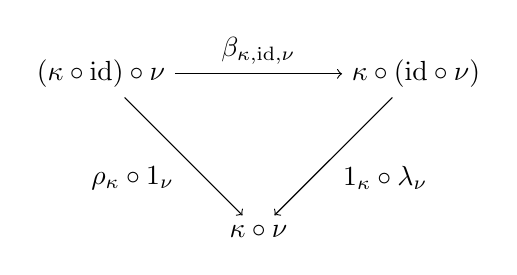
\begin{tikzpicture}[scale=2]
    \node (P1) at (-1,1) {$(\kappa \circ \mathrm{id})\circ \nu$};
    \node (P2) at (1,1) {$\kappa \circ (\mathrm{id}\circ \nu)$};
    \node (P3) at (0,0) {$\kappa \circ \nu$};
    \draw[->] (P1)--(P2) node[midway,above] {$\beta_{\kappa,\mathrm{id},\nu}$};
    \draw[->] (P1)--(P3) node[midway,below left] {$\rho_\kappa\circ 1_\nu$};
    \draw[->] (P2)--(P3) node[midway,below right] {$1_\kappa \circ \lambda_\nu$};
\end{tikzpicture} \quad \quad 
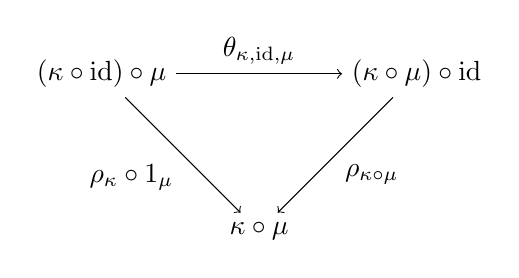
\begin{tikzpicture}[scale=2]
    \node (P1) at (-1,1) {$(\kappa \circ \mathrm{id})\circ \mu$};
    \node (P2) at (1,1) {$(\kappa\circ \mu)\circ\mathrm{id}$};
    \node (P3) at (0,0) {$\kappa \circ \mu$};
    \draw[->] (P1)--(P2) node[midway,above] {$\theta_{\kappa,\mathrm{id},\mu}$};
    \draw[->] (P1)--(P3) node[midway,below left] {$\rho_\kappa\circ 1_\mu$};
    \draw[->] (P2)--(P3) node[midway,below right] {$\rho_{\kappa\circ\mu}$};
\end{tikzpicture} \quad \ ,
\end{center}
pentagonal \\
\resizebox{\linewidth}{!}{
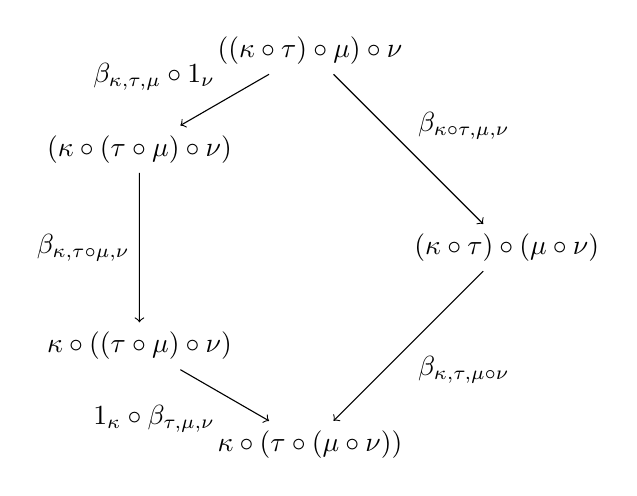
\begin{tikzpicture}[scale=2.5]
    \node (P1) at (0,1) {$((\kappa\circ\tau)\circ\mu)\circ\nu$};
    \node (P2) at (-0.866,0.5) {$(\kappa\circ(\tau\circ\mu)\circ\nu)$};
    \node (P3) at (-0.866,-0.5) {$\kappa\circ((\tau\circ\mu)\circ\nu)$};
    \node (P4) at (0,-1) {$\kappa\circ(\tau\circ(\mu\circ\nu))$};
    \node (P5) at (1,0) {$(\kappa\circ\tau)\circ(\mu\circ\nu)$} ;
    \draw[->] (P1)--(P2) node[midway,above left] {$\beta_{\kappa,\tau,\mu}\circ 1_\nu$};
    \draw[->] (P2)--(P3) node[midway,left] {$\beta_{\kappa,\tau\circ\mu,\nu}$};
    \draw[->] (P3)--(P4) node[midway,below left] {$1_\kappa \circ \beta_{\tau,\mu,\nu}$};
    \draw[->] (P1)--(P5) node[midway,above right] {$\beta_{\kappa\circ\tau,\mu,\nu}$};
    \draw[->] (P5)--(P4) node[midway,below right] {$\beta_{\kappa,\tau,\mu\circ\nu}$};
\end{tikzpicture} \quad 
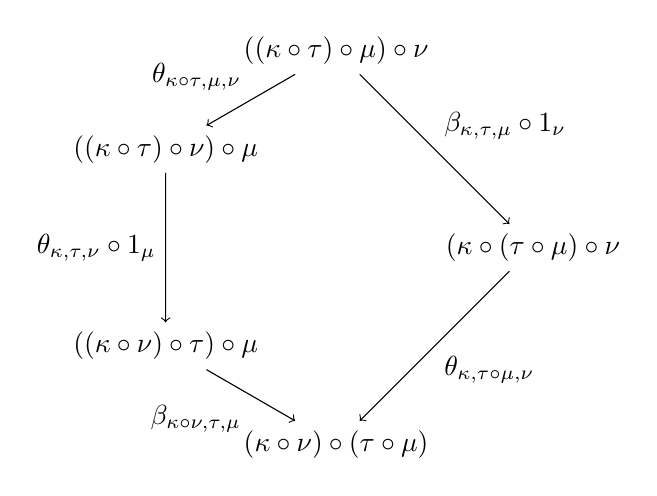
\begin{tikzpicture}[scale=2.5]
    \node (P1) at (0,1) {$((\kappa\circ\tau)\circ\mu)\circ\nu$};
    \node (P2) at (-0.866,0.5) {$((\kappa\circ\tau)\circ\nu)\circ\mu$};
    \node (P3) at (-0.866,-0.5) {$((\kappa\circ\nu)\circ\tau)\circ\mu$};
    \node (P4) at (0,-1) {$(\kappa\circ\nu)\circ(\tau\circ\mu)$};
    \node (P5) at (1,0) {$(\kappa\circ(\tau\circ\mu)\circ\nu$} ;
    \draw[->] (P1)--(P2) node[midway,above left] {$\theta_{\kappa\circ\tau,\mu,\nu}$};
    \draw[->] (P2)--(P3) node[midway,left] {$\theta_{\kappa,\tau,\nu}\circ 1_\mu$};
    \draw[->] (P3)--(P4) node[midway,below left] {$\beta_{\kappa\circ\nu,\tau,\mu}$};
    \draw[->] (P1)--(P5) node[midway,above right] {$\beta_{\kappa,\tau,\mu}\circ 1_\nu$};
    \draw[->] (P5)--(P4) node[midway,below right] {$\theta_{\kappa,\tau\circ\mu,\nu}$};
\end{tikzpicture} \quad 
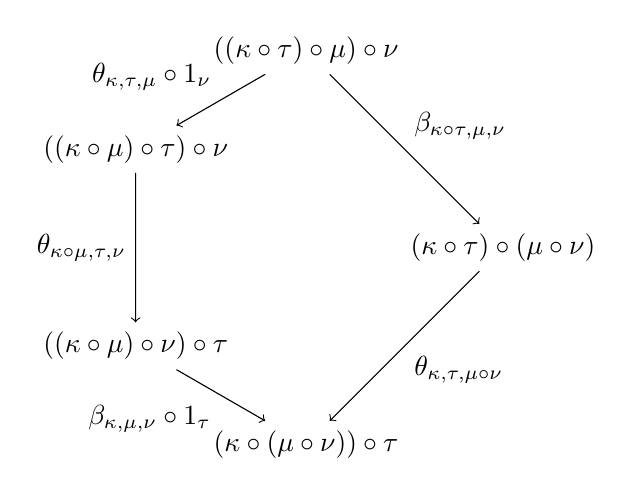
\begin{tikzpicture}[scale=2.5]
    \node (P1) at (0,1) {$((\kappa\circ\tau)\circ\mu)\circ\nu$};
    \node (P2) at (-0.866,0.5) {$((\kappa\circ\mu)\circ\tau)\circ\nu$};
    \node (P3) at (-0.866,-0.5) {$((\kappa\circ\mu)\circ\nu)\circ\tau$};
    \node (P4) at (0,-1) {$(\kappa\circ(\mu\circ\nu))\circ\tau$};
    \node (P5) at (1,0) {$(\kappa\circ\tau)\circ(\mu\circ\nu)$} ;
    \draw[->] (P1)--(P2) node[midway,above left] {$\theta_{\kappa,\tau,\mu}\circ 1_\nu$};
    \draw[->] (P2)--(P3) node[midway,left] {$\theta_{\kappa\circ\mu,\tau,\nu}$};
    \draw[->] (P3)--(P4) node[midway,below left] {$\beta_{\kappa,\mu,\nu}\circ 1_\tau$};
    \draw[->] (P1)--(P5) node[midway,above right] {$\beta_{\kappa\circ\tau,\mu,\nu}$};
    \draw[->] (P5)--(P4) node[midway,below right] {$\theta_{\kappa,\tau,\mu\circ\nu}$};
\end{tikzpicture} } \\
and hexagonal identities \\
\begin{center}
\resizebox{0.8\linewidth}{!}{
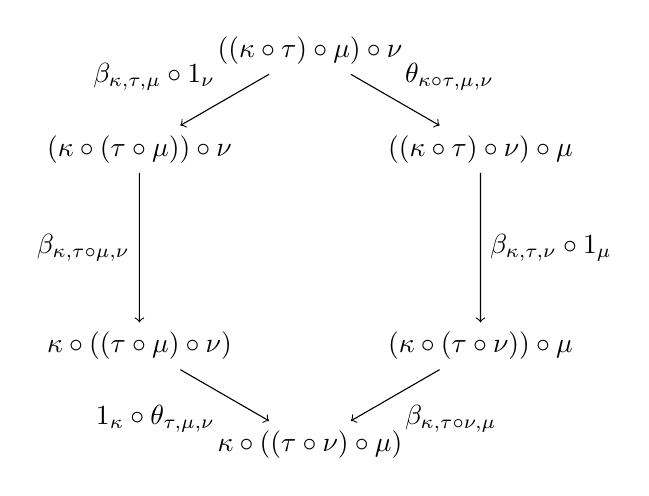
\begin{tikzpicture}[scale=2.5]
    \node (P1) at (0,1) {$((\kappa\circ\tau)\circ\mu)\circ\nu$};
    \node (P2) at (-0.866,0.5) {$(\kappa\circ(\tau\circ\mu))\circ\nu$};
    \node (P3) at (-0.866,-0.5) {$\kappa\circ((\tau\circ\mu)\circ\nu)$};
    \node (P4) at (0,-1) {$\kappa\circ((\tau\circ\nu)\circ\mu)$};
    \node (P5) at (0.866,0.5) {$((\kappa\circ\tau)\circ\nu)\circ\mu$} ;
    \node (P6) at (0.866,-0.5) {$(\kappa\circ(\tau\circ\nu))\circ\mu$};
    \draw[->] (P1)--(P2) node[midway,above left] {$\beta_{\kappa,\tau,\mu}\circ 1_\nu$};
    \draw[->] (P2)--(P3) node[midway,left] {$\beta_{\kappa,\tau\circ\mu,\nu}$};
    \draw[->] (P3)--(P4) node[midway,below left] {$1_\kappa \circ \theta_{\tau,\mu,\nu}$};
    \draw[->] (P1)--(P5) node[midway,above right] {$\theta_{\kappa\circ\tau,\mu,\nu}$};
    \draw[->] (P5)--(P6) node[midway,right] {$\beta_{\kappa,\tau,\nu}\circ 1_\mu$};
    \draw[->] (P6)--(P4) node[midway,below right] {$\beta_{\kappa,\tau\circ\nu,\mu}$};
\end{tikzpicture} \quad \quad
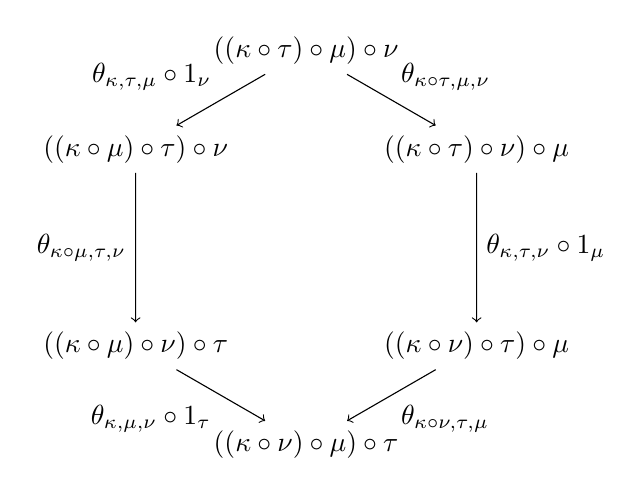
\begin{tikzpicture}[scale=2.5]
    \node (P1) at (0,1) {$((\kappa\circ\tau)\circ\mu)\circ\nu$};
    \node (P2) at (-0.866,0.5) {$((\kappa\circ\mu)\circ\tau)\circ\nu$};
    \node (P3) at (-0.866,-0.5) {$((\kappa\circ\mu)\circ\nu)\circ\tau$};
    \node (P4) at (0,-1) {$((\kappa\circ\nu)\circ\mu)\circ\tau$};
    \node (P5) at (0.866,0.5) {$((\kappa\circ\tau)\circ\nu)\circ\mu$} ;
    \node (P6) at (0.866,-0.5) {$((\kappa\circ\nu)\circ\tau)\circ\mu$};
    \draw[->] (P1)--(P2) node[midway,above left] {$\theta_{\kappa,\tau,\mu}\circ 1_\nu$};
    \draw[->] (P2)--(P3) node[midway,left] {$\theta_{\kappa\circ\mu,\tau,\nu}$};
    \draw[->] (P3)--(P4) node[midway,below left] {$\theta_{\kappa,\mu,\nu}\circ 1_\tau$};
    \draw[->] (P1)--(P5) node[midway,above right] {$\theta_{\kappa\circ\tau,\mu,\nu}$};
    \draw[->] (P5)--(P6) node[midway,right] {$\theta_{\kappa,\tau,\nu}\circ 1_\mu$};
    \draw[->] (P6)--(P4) node[midway,below right] {$\theta_{\kappa\circ\nu,\tau,\mu}$};
\end{tikzpicture}  } \quad \ .
\end{center}
\end{definition}

A categorified ns operad concentrated in arity 1 is a monoidal category.




\subsection{Coherence for categorified operads}

Recall from [REF] the definition of the $\mathbb{N}$-colored operad $\mathcal{O}$ encoding ns operads. Its minimal resolution is given by the cellular chains on the operahedra [DEF]. 


\begin{thm}[Coherence theorem] \label{thm:coherence}
    Every diagram with vertices iterates of the $\circ_i$ and edges expansions of instances of $\beta, \theta, \lambda$ and $\rho$ arrows is commutative. 
\end{thm}

\begin{proof} TBC
\end{proof}

Restricted to categorified ns operad concentrated in arity 1, i.e. to monoidal categories, we recover MacLane's original coherence tbeorem [REF].

There is an analogous statement for weak Cat-operads \cite[Proposition 14.2]{DP15}. In the same fashion as for \cref{thm:equivalenceDPGLA}, one can prove that the two statements are equivalent. 


\subsection{Weak Cat-operads}

\begin{definition}[Weak Cat-operad {\cite{DP15}}]
\end{definition}

\begin{thm} \label{thm:equivalenceDPGLA}
    The data of a categorified ns operad and the data of a weak Cat-operad are equivalent.  
\end{thm}

\begin{proof}
    TBC
\end{proof}



